\documentclass[10pt,twocolumn]{article}
\usepackage[margin=1in]{geometry}
\usepackage[T1]{fontenc}
\usepackage{times}
\usepackage{amsmath}
\usepackage{graphicx}
\usepackage{booktabs}
\usepackage{url}
\graphicspath{{figures/}}
\setlength{\textfloatsep}{8pt}
\setlength{\floatsep}{6pt}

\title{Tabular Q-Learning and Deep Q-Networks on Gymnasium:\\A Controlled Comparison on CartPole and a DQN Study on LunarLander}
\author{Ismael Paredes}
\date{November 2026}

\begin{document}
\maketitle

\begin{abstract}
We implement tabular Q-learning and Deep Q-Networks (DQN) from scratch and compare them on CartPole-v1 under the same budget of 200k environment steps, the same exploration schedule and five seeds. No tabular configuration reached the success threshold of 475, with the best reaching a mean of 311.0, whereas DQN reached it on all five seeds with a mean of 498.9, at about seven times the training time. We also report a failure that we did not expect: with a Huber loss, DQN's value estimates exceeded the true maximum of 100 and its final return was only 72.7, while changing the loss alone to mean squared error removed the problem. On LunarLander-v3, the base DQN reached the threshold of 200 on all three seeds, with a mean of 252.9. Removing the replay buffer prevented learning ($-34.6$), while removing the target network changed little (234.9), which we did not expect.
\end{abstract}

\section{Introduction}
Reinforcement learning methods differ in what kind of problem they can represent. Tabular methods store one value per state and action, so they need a small or discretizable state space. DQN \cite{mnih2015} replaces the table with a neural network and handles continuous observations, but it still needs a discrete action space. This project tests those limits in practice.

We make three contributions. First, a comparison of tabular Q-learning and DQN on CartPole-v1 \cite{towers2024}, on the same axes and step budget, including the effect of the number and range of bins. Second, a DQN study on LunarLander-v3, with a hyperparameter study of learning rate and exploration, and an ablation of the target network and the replay buffer. Third, a diagnosis of a divergence that appeared while building the DQN agent. A written analysis explains why other Gymnasium tasks suit neither method.

\section{Pertinence Analysis}
\textbf{CartPole-v1} has 4 continuous observations and 2 actions. Four dimensions can be discretized: 10 bins per dimension give $10^4$ states, a table small enough to fill with 200k steps. It therefore suits both methods. Two of its dimensions (the velocities) are unbounded, so a discretization must choose its limits.

\textbf{LunarLander-v3} has 8 observations and 4 actions. Discretization scales poorly here: 10 bins per dimension give $10^8$ states, or $4\times10^8$ table entries, far more than the 500k transitions in our budget. Most states would never be visited. The action space is discrete, however, so DQN applies directly.

\section{Methods}
\subsection{Discretization and Q-Learning}
Each observation dimension is split into $n$ equal-width bins between chosen limits, and values outside the limits fall into the outer bins. Position and angle use the limits at which CartPole terminates ($\pm2.4$ and $\pm0.2095$). For the velocities we measured 100k observations under a random policy, whose 0.5th and 99.5th percentiles are about $\pm1.5$ for the cart and $\pm2.0$ for the pole, and used those as the base limits. The agent applies the standard update \cite{sutton2018}
\begin{equation}
Q(s,a) \leftarrow Q(s,a) + \alpha\big[r + \gamma \max_{a'} Q(s',a') - Q(s,a)\big]
\end{equation}
with $\alpha=0.1$ and $\gamma=0.99$. While training, ties between equal action values are broken at random, so that unvisited states do not always choose the first action.

\subsection{DQN}
The Q-network is a multilayer perceptron with two hidden layers of 128 ReLU units, trained with Adam. Transitions go into a circular replay buffer. Every 4 environment steps, a batch of 64 transitions is sampled uniformly and the network is trained towards
\begin{equation}
y = r + \gamma\,(1-d)\,\max_{a'} Q_{\bar\theta}(s',a'),
\end{equation}
where $Q_{\bar\theta}$ is a target network copied from the online network every 500 steps. In both agents $d=1$ only when the environment terminates. An episode cut by the time limit still bootstraps, because the state it stopped in has future value. Exploration is $\varepsilon$-greedy, with $\varepsilon$ decaying linearly from 1 to 0.05.

The two ablations keep the number and size of gradient updates unchanged. Without a target network, $Q_{\bar\theta}$ is the online network itself. Without replay, the buffer holds only the latest 64 transitions, so samples are recent and correlated.

\section{Experimental Settings}
All runs use Gymnasium 1.4.0 and PyTorch 2.15 on an Intel i5-8300H CPU (4 cores, 11.8 GB of RAM), with four runs in parallel and one thread each. Each result uses fixed seeds for the environment, NumPy and PyTorch; repeating a seed reproduces the logs exactly. Training all 61 reported runs took 2.56 CPU hours.

Evaluation is separate from training. At regular intervals (5k steps on CartPole, 10k on LunarLander) we run 10 greedy episodes in a separate environment with fixed start seeds. After training, 100 greedy episodes on the final weights decide whether the threshold is met. Figures show the mean across seeds with a band of one standard deviation, clipped to the range the metric can take. Training time excludes evaluation.

\textbf{Tier 1} uses 200k steps and 5 seeds. Tabular configurations use 6, 10 and 20 bins, plus 10 bins with velocity limits halved (narrow) and doubled (wide). Both methods share one schedule, with $\varepsilon$ reaching 0.05 at 100k steps.

\textbf{Tier 2} uses 500k steps and 3 seeds. The base configuration has a learning rate of $5\times10^{-4}$, a buffer of 100k transitions and $\varepsilon$ reaching 0.05 at 50k steps. We vary one parameter at a time: learning rate ($2.5\times10^{-4}$, $5\times10^{-4}$, $10^{-3}$) and the $\varepsilon$ decay length (25k, 50k, 100k), then remove the target network or the replay buffer. This makes 7 configurations and 21 runs.

Table~\ref{tab:params} lists the settings. We kept them fixed unless stated otherwise. The full configuration of each experiment is stored as a YAML file in the repository.

\begin{table}[t]
\centering\small
\caption{Base hyperparameters.}
\label{tab:params}
\begin{tabular}{lrr}
\toprule
Parameter & CartPole & LunarLander \
\midrule
Environment steps & 200k & 500k \
Seeds & 5 & 3 \
Discount $\gamma$ & 0.99 & 0.99 \
$\varepsilon$ start, end & 1, 0.05 & 1, 0.05 \
$\varepsilon$ decay steps & 100k & 50k \
\midrule
\multicolumn{3}{l}{\emph{DQN}} \
Hidden layers & 128, 128 & 128, 128 \
Learning rate & $5\times10^{-4}$ & $5\times10^{-4}$ \
Loss & MSE & MSE \
Buffer size & 50k & 100k \
Batch size & 64 & 64 \
Training interval & 4 steps & 4 steps \
Target update interval & 500 steps & 500 steps \
Learning starts & 1,000 steps & 1,000 steps \
\midrule
\multicolumn{3}{l}{\emph{Tabular}} \
Step size $\alpha$ & 0.1 & -- \
Initial Q-values & 0 & -- \
\bottomrule
\end{tabular}
\end{table}

\section{Results}
\subsection{Tier 1: Tabular Q-Learning}
Table~\ref{tab:tabular} and Figure~\ref{fig:tabular} show that every configuration learned, compared with a random policy's return of 22.6, but none reached 475 in the final evaluation. With 20 bins, learning started later and ended higher. The narrow limits matched 20 bins with half the resolution per dimension, and reached 475 in at least one 10-episode evaluation on 3 of 5 seeds. The differences are small relative to the spread across seeds: 6 and 10 bins cannot be told apart.

\begin{table}[t]
\centering\small
\caption{Tabular results on CartPole (5 seeds). Final return is the mean $\pm$ standard deviation across seeds. ``Hit'' counts seeds with any 10-episode evaluation of at least 475. No seed reached 475 in the final evaluation.}
\label{tab:tabular}
\begin{tabular}{lrrr}
\toprule
Configuration & Final return & Hit & Visited \\
\midrule
6 bins & 235.4 $\pm$ 65.5 & 0 & 39.3\% \\
10 bins & 253.3 $\pm$ 86.5 & 2 & 17.1\% \\
20 bins & 311.0 $\pm$ 65.5 & 0 & 2.9\% \\
10 bins, narrow & 310.3 $\pm$ 119.7 & 3 & 11.7\% \\
10 bins, wide & 247.0 $\pm$ 124.8 & 1 & 11.5\% \\
\bottomrule
\end{tabular}
\end{table}

\begin{figure}[t]
\centering
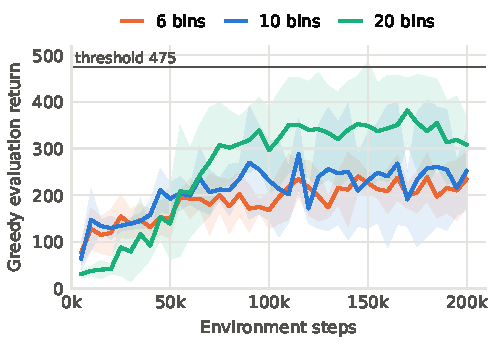
\includegraphics[width=\columnwidth]{tier1_tabular_bins.pdf}\\[2pt]
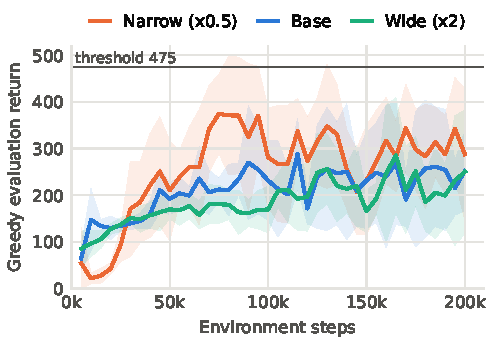
\includegraphics[width=\columnwidth]{tier1_tabular_ranges.pdf}
\caption{Tabular Q-learning on CartPole: effect of the number of bins (top) and of the velocity limits with 10 bins (bottom).}
\label{fig:tabular}
\end{figure}

\subsection{Tier 1: Tabular versus DQN}
DQN reached the threshold on all 5 seeds, with a final return of $498.9 \pm 2.4$ against $311.0 \pm 65.5$ for the best tabular configuration (Figure~\ref{fig:compare}). The order changed during training. Mean evaluation return favoured DQN until about 65k steps, the tabular agent from there to about 125k, and DQN afterwards. The median first evaluation at or above 475 was at 115k steps.

Measured in time, the result is different: a tabular run took 20.1 s and a DQN run 135.6 s. The tabular agent first averaged 300 after 6.0 s, and DQN held that level from 77.7 s. Table~\ref{tab:compare} summarizes both methods.

\begin{table}[t]
\centering\small
\caption{Tier 1 comparison (5 seeds, 200k steps). ``Pass'' counts seeds at or above 475 in the final evaluation. ``Steps'' is the median first 10-episode evaluation at or above 475, among seeds that had one.}
\label{tab:compare}
\begin{tabular}{lrrrr}
\toprule
Method & Final return & Pass & Steps & Time \\
\midrule
Tabular, 20 bins & 311.0 $\pm$ 65.5 & 0 & none & 20 s \\
Tabular, narrow & 310.3 $\pm$ 119.7 & 0 & 90k & 23 s \\
DQN, MSE & 498.9 $\pm$ 2.4 & 5 & 115k & 136 s \\
DQN, Huber & 72.7 $\pm$ 32.4 & 0 & none & 125 s \\
\bottomrule
\end{tabular}
\end{table}

\begin{figure}[t]
\centering
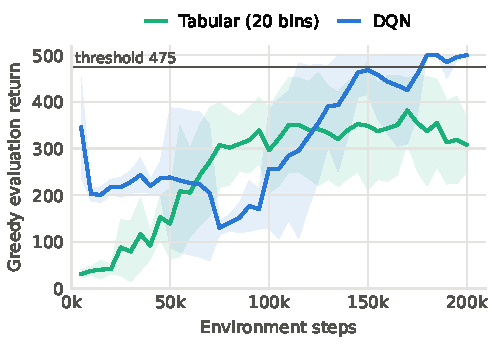
\includegraphics[width=\columnwidth]{tier1_compare_steps.pdf}\\[2pt]
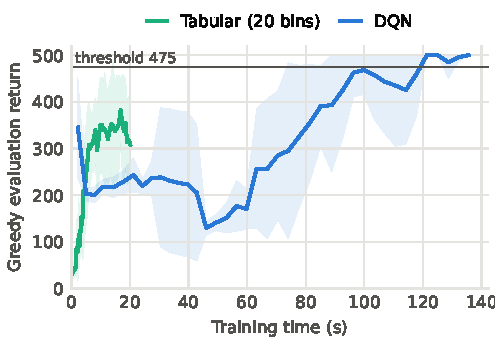
\includegraphics[width=\columnwidth]{tier1_compare_time.pdf}
\caption{Tabular Q-learning and DQN on CartPole, against environment steps (top) and training time (bottom).}
\label{fig:compare}
\end{figure}

\subsection{Tier 1: A Divergence Caused by the Loss}
Our first DQN used a Huber loss. Its mean Q-value rose past 100, the highest value possible with a reward of 1 and $\gamma=0.99$, since $1/(1-\gamma)=100$. It peaked between 202 and 1564 depending on the seed (Figure~\ref{fig:loss}), and the final return was $72.7 \pm 32.4$, with no seed near the threshold. Changing only the loss to mean squared error gave the results above, with peaks of 110 to 140.

To rule out a bug, we added a test on a three-state chain with known optimal values, and the agent recovers them. Slow exploration was our first suspect, since it keeps the data far from the greedy policy for longer. But MSE succeeded with the same slow schedule, so exploration was not the main cause. The schedule does matter for the tabular agent, whose final return fell to $136.9 \pm 77.2$ with a 20k decay, so we kept 100k for both methods.

\begin{figure}[t]
\centering
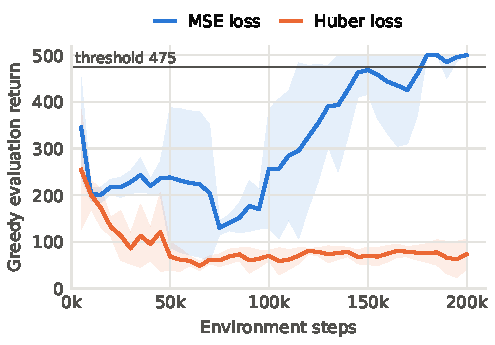
\includegraphics[width=\columnwidth]{tier1_loss_return.pdf}\[2pt]
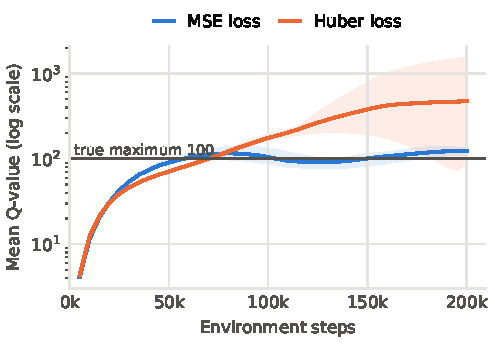
\includegraphics[width=\columnwidth]{tier1_loss_q.pdf}
\caption{DQN on CartPole with MSE and Huber losses: evaluation return (top) and mean Q-value on a log scale (bottom). In the bottom panel, bands show the minimum and maximum across seeds.}
\label{fig:loss}
\end{figure}

\subsection{Tier 2: DQN on LunarLander}
The base DQN reached the threshold on all 3 seeds, with a final return of $252.9 \pm 15.5$ (Table~\ref{tab:tier2}). Its first evaluation at or above 200 came at a median of 250k steps, although the mean across seeds only reached that level at about 330k. Learning was slow and uneven: mean return stayed near or below zero for most of the first 200k steps, before the agent started to land reliably.

\begin{table}[t]
\centering\small
\caption{LunarLander results (3 seeds, 500k steps). ``Pass'' counts seeds at or above 200 in the final 100-episode evaluation. ``Steps'' is the median first evaluation at or above 200.}
\label{tab:tier2}
\begin{tabular}{lrrr}
\toprule
Configuration & Final return & Pass & Steps \\
\midrule
Base & 252.9 $\pm$ 15.5 & 3 & 250k \\
lr $2.5\times10^{-4}$ & 175.3 $\pm$ 60.5 & 2 & 380k \\
lr $10^{-3}$ & 257.6 $\pm$ 3.8 & 3 & 270k \\
$\varepsilon$ decay 25k & 224.0 $\pm$ 15.1 & 3 & 350k \\
$\varepsilon$ decay 100k & 258.0 $\pm$ 22.0 & 3 & 220k \\
No target network & 234.9 $\pm$ 2.2 & 3 & 360k \\
No replay buffer & $-34.6 \pm$ 24.0 & 0 & -- \\
\bottomrule
\end{tabular}
\end{table}

\textbf{Hyperparameters.} The lowest learning rate was the only setting to miss the threshold on any seed, and it reached 200 later than the others (Figure~\ref{fig:tier2study}). Its mean Q-value was also far lower at the end (33.9 against 76.0), which fits slow learning rather than instability. Doubling the rate gave a similar result to the base. The three $\varepsilon$ schedules all passed. The shortest decay gave the lowest return of the three and the longest the highest, but with 3 seeds these gaps are within the spread of the results.

\begin{figure}[t]
\centering
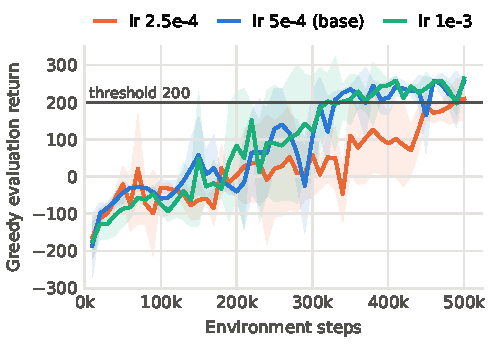
\includegraphics[width=\columnwidth]{tier2_lr.pdf}\\[2pt]
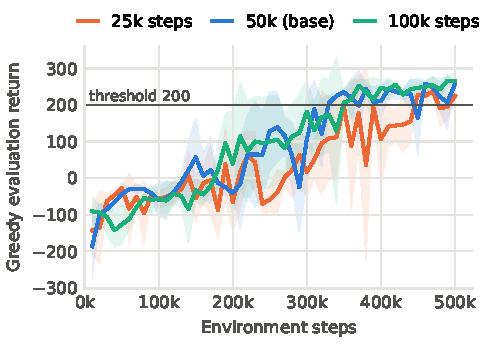
\includegraphics[width=\columnwidth]{tier2_eps.pdf}
\caption{DQN on LunarLander: learning rate (top) and length of the $\varepsilon$ decay (bottom).}
\label{fig:tier2study}
\end{figure}

\textbf{Ablation.} Without replay, no seed came near the threshold: final return was $-34.6 \pm 24.0$ and the mean curve stayed below zero throughout (Figure~\ref{fig:ablation}). Without a target network, all 3 seeds passed with $234.9 \pm 2.2$. Their median first evaluation at 200 came later (360k against 250k steps), and mean Q-values stayed in a normal range, with peaks of 64 to 84 against 75 to 78 for the base. We saw no divergence.

\begin{figure}[t]
\centering
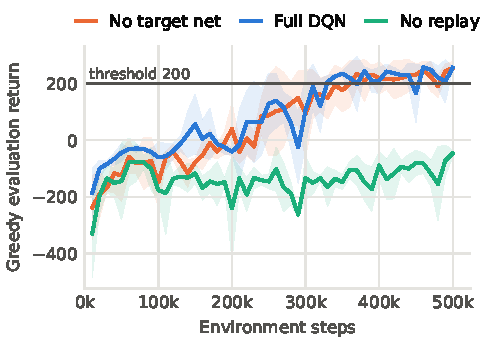
\includegraphics[width=\columnwidth]{tier2_ablation.pdf}
\caption{Ablation on LunarLander: full DQN, no target network and no replay buffer.}
\label{fig:ablation}
\end{figure}

\subsection{Compute and Qualitative Evidence}
A LunarLander run took between 307 s and 393 s of training on average, depending on the configuration. The repository includes GIFs of trained agents. On one episode each, the DQN agent balanced CartPole for the full 500 steps, the 20-bin tabular agent lasted 341 steps, and the base LunarLander agent landed with a return of 283. These single episodes illustrate the policies and are not additional measurements.

\section{Discussion}
\textbf{Which method learned faster in Tier 1?} It depends on the measure. Per step, neither led throughout, but only DQN kept improving past the tabular plateau. A table updates one entry per transition and cannot generalize: each new bin starts from zero, which suits early learning at coarse resolution and limits final precision. A network shares information between similar states and reuses each transition through replay, at a higher cost per step. Per second, the tabular agent wins early by a wide margin, because its update is a single array operation.

\textbf{How sensitive was each method to its key design choice?} For the tabular agent, the visited share of the table explains the trade-off. It fell from 39.3\% with 6 bins to 2.9\% with 20, which is still more states in absolute terms (about 510 against 4,600). More bins bring precision at the price of more states to fill. The narrow limits suggest that where the bins lie matters as much as how many there are: a hand-written balancing controller stays within about $\pm0.05$ rad and $\pm0.3$ rad/s, a small region that wide uniform bins cover with very few cells. We have not verified this explanation directly. DQN's most critical choice in Tier 1 was the loss, which separated complete success from failure. On LunarLander, the learning rate mattered most among the parameters we varied: halving it cost about 78 points of mean return, while doubling it or changing the exploration schedule stayed within about 30 points of the base.

\textbf{Why did Huber diverge?} Off-policy data, bootstrapping and function approximation form the ``deadly triad'', which can cause divergence \cite{sutton2018,vanhasselt2018}. Our proposed mechanism is specific to CartPole. All rewards are $+1$, so the only force pulling values down is the terminal transition, whose target is 1 while the prediction is near 100. Those are exactly the transitions with very large errors, and Huber limits their gradient to the same size as any other, while MSE lets it grow with the error. This is an explanation consistent with the data, not something we measured. It also does not show that Huber is a poor choice in general, and the original DQN clips errors in a similar way \cite{mnih2015}.

\textbf{What did the ablation reveal?} Replay was essential here and the target network was not, which is not the order we expected. Without replay, the agent learns only from its last 64 transitions. They are highly correlated and all come from one part of one trajectory, so each update fits the current situation and can overwrite what was learned about others. A landing episode moves through very different phases, from descent to touchdown, which may make this especially harmful. The fall of the mean Q-value is consistent with that picture, from peaks of 38 to 44 to about 10 at the end.

The small effect of the target network needs care. Its purpose is to keep targets steady \cite{mnih2015}, and our result does not show it is unnecessary in general. A possible reason is that updates here are small and infrequent, with a learning rate of $5\times10^{-4}$ every 4 steps, so the online network may already change slowly. We did not test this. The ablation used 3 seeds on one low-dimensional task, and the later median arrival at 200 suggests a cost in speed that more seeds could confirm. We also did not test Huber on LunarLander, so the Tier 1 loss result should not be extended to it.

\textbf{Limitations.} The comparison is not fully symmetric. We selected the loss after looking at seeds 0 and 1, which are also among the reported seeds, and the tabular agent received no equivalent tuning beyond the exploration check. DQN also remained unstable: two seeds fell to about 126 at some point after reaching 500, and one seed averaged 388.8 over its last 10 evaluations despite finishing at 500, so final scores depend partly on when training stops. With 3 to 5 seeds, small differences should not be read as real effects. Evaluations of 10 episodes are noisy, which is why we use 100 episodes for the threshold. Training times were measured with four runs sharing the CPU. On LunarLander, the base was not tuned: two variants ended slightly above it. We raised the budget to 500k steps after seeing three base runs at 300k (final returns of 123.0, 236.3 and 35.0, still rising), and restarted every configuration so that all share the same budget.

\section{Analysis-Only Component}
\textbf{Why continuous control does not suit these methods.} Tabular Q-learning and DQN both select actions with a maximum over all actions, so they need a finite and reasonably small set of actions. BipedalWalker and the MuJoCo locomotion tasks have continuous multi-joint actions. Discretizing each joint separately makes the number of joint actions grow exponentially (Table~\ref{tab:actions}).

\begin{table}[t]
\centering\small
\caption{Size of the action set after discretizing each action dimension. Dimensions come from Gymnasium (v5 for MuJoCo, v3 for BipedalWalker).}
\label{tab:actions}
\begin{tabular}{lrrrr}
\toprule
Task & Obs. & Act. & 5 bins & 11 bins \\
\midrule
Hopper & 11 & 3 & 125 & 1,331 \\
BipedalWalker & 24 & 4 & 625 & 14,641 \\
HalfCheetah & 17 & 6 & 15,625 & 1,771,561 \\
Ant & 105 & 8 & 390,625 & 214,358,881 \\
\bottomrule
\end{tabular}
\end{table}

A DQN output layer for Ant with 11 bins per joint would need more than 214 million units, and the maximum in the target would run over all of them. Each output is also trained only when its action is sampled, so nearly all would never be updated. Coarse bins do not solve this: 5 bins still give 390,625 actions, and they remove the fine torque control that locomotion depends on. Hopper at 5 bins is the only entry that looks manageable, and it would still lose that precision.

The observations rule out tables as well. BipedalWalker has 24 dimensions, so even 5 bins per dimension give $5^{24}\approx6\times10^{16}$ states, and Ant's 105 dimensions make the count meaningless. DQN handles such observations, so for these tasks the obstacle is the action space alone.

\textbf{Which algorithms suit these tasks.} Methods that represent the policy directly avoid the maximum over actions. PPO \cite{schulman2017} is an on-policy policy-gradient method: a network outputs the parameters of a continuous action distribution, and a clipped objective limits each update. It is simple and stable, but its on-policy data is used for only a few updates, so it needs many environment steps. SAC \cite{haarnoja2018} and TD3 \cite{fujimoto2018} are off-policy actor-critic methods. An actor network proposes the action, which replaces the maximum in the critic's target, and replay buffers reuse past data, which tends to make them more sample-efficient. SAC adds an entropy term that encourages exploration. TD3 uses two critics to reduce overestimation, the same bias family seen in our Q-values, and delays policy updates.

\textbf{Why tabular methods fail on pixels.} An Atari frame has $210\times160$ pixels with 3 color channels, or 100,800 values of 256 levels each. Even after the usual preprocessing to four stacked $84\times84$ grayscale frames, an observation has 28,224 values, so the number of possible states is $256^{28224}$. A table cannot store this, and storage is not the main obstacle. An exact table never generalizes, and two frames that differ in one pixel are different states with no shared knowledge, so almost every state would be new. Discretizing pixels does not help, because the relevant information (object positions and velocities) is not aligned with any pixel-level grid. Convolutional networks in DQN \cite{mnih2015} address this by learning features that are shared across similar frames.

\section{AI-Use Statement}
This project used Claude Code (Claude Opus 5.5, Anthropic) for planning, writing code and tests, debugging, drafting this paper and verifying references. The student chose the environments and scope, and is responsible for all submitted work. Results come from running the code in this repository, and each figure and table can be regenerated with the commands in its README. References were checked online, and those whose venue could not be confirmed are cited as preprints. An initial AI explanation for the DQN divergence (slow exploration) proved wrong as the main cause when tested, and the paper reports the controlled result. Appendix~\ref{app:prompts} lists the main prompts, and \texttt{report/ai\_use.md} holds the full log.

\begin{thebibliography}{9}\small
\bibitem{fujimoto2018} S. Fujimoto, H. van Hoof, and D. Meger. Addressing function approximation error in actor-critic methods. arXiv:1802.09477, 2018.
\bibitem{haarnoja2018} T. Haarnoja, A. Zhou, P. Abbeel, and S. Levine. Soft actor-critic: Off-policy maximum entropy deep reinforcement learning with a stochastic actor. arXiv:1801.01290, 2018.
\bibitem{mnih2015} V. Mnih et al. Human-level control through deep reinforcement learning. \emph{Nature}, 518:529--533, 2015.
\bibitem{schulman2017} J. Schulman, F. Wolski, P. Dhariwal, A. Radford, and O. Klimov. Proximal policy optimization algorithms. arXiv:1707.06347, 2017.
\bibitem{sutton2018} R. S. Sutton and A. G. Barto. \emph{Reinforcement Learning: An Introduction}. MIT Press, 2nd edition, 2018.
\bibitem{towers2024} M. Towers et al. Gymnasium: A standard interface for reinforcement learning environments. arXiv:2407.17032, 2024.
\bibitem{vanhasselt2018} H. van Hasselt, Y. Doron, F. Strub, M. Hessel, N. Sonnerat, and J. Modayil. Deep reinforcement learning and the deadly triad. arXiv:1812.02648, 2018.
\end{thebibliography}

\appendix
\section{Main Prompts}
\label{app:prompts}
\small
\begin{enumerate}
\item The full project brief, followed by: ``I have to do this project. I am doing it individually. For each important decision, ask me if necessary.'' (translated from Spanish).
\item Scope answers given by the student: CartPole-v1 for Tier 1, LunarLander-v3 for Tier 2, no Tier 3, Claude writes the code and the student reviews it by stage, paper in English with LaTeX.
\item ``Continue'' at the end of each stage, after Claude reported its results.
\item A note that only about two hours remained, which led to merging the LunarLander pilot into the main runs.
\end{enumerate}

\end{document}
